\chapter{Simetri dan Grup Titik}\label{ch:b3:point-groups}

Putarlah sebuah kristal salju sebesar enam puluh derajat dan tidak ada yang
berubah; putarlah molekul benzena dengan sudut yang sama, maka keenam karbon
dan keenam hidrogennya tepat menempati tempat satu sama lain. Simetri sebuah
molekul menentukan beberapa sifatnya sebelum perhitungan apa pun: apakah
molekul itu dapat mempunyai momen dipol, apakah molekul itu dapat berada
dalam dua bentuk yang saling bayangan cermin, vibrasi mana yang menyerap
cahaya inframerah, orbital mana yang boleh bercampur. Untuk memanfaatkannya,
para kimiawan meminjam bahasa grup dari matematika. Bab ini mendefinisikan
\omterm{def:b3:point-groups:operation}{operasi-operasi simetri} sebuah molekul, menghimpunnya menjadi \omterm{def:b3:point-groups:point-group}{grup titiknya},
memberikan prosedur untuk menemukan grup itu, membuktikan dua teorema tentang
kepolaran dan kiralitas, dan memperkenalkan tabel-tabel \omterm{def:b3:point-groups:representation}{karakter} yang menjadi
landasan \cref{ch:b3:group-theory-applied}.

\begin{recall}
Jilid Tahun 1 meramalkan bentuk molekul dengan model VSEPR, mendefinisikan
momen dipol molekul polar, dan mendefinisikan kiralitas: molekul kiral tidak
dapat ditumpangtindihkan dengan bayangan cerminnya. Jilid Tahun 2 memakai
simetri secara deskriptif untuk menyusun orbital-orbital fragmen \ce{H2O} dan
\ce{NH3}.
\end{recall}

\begin{omfigure}
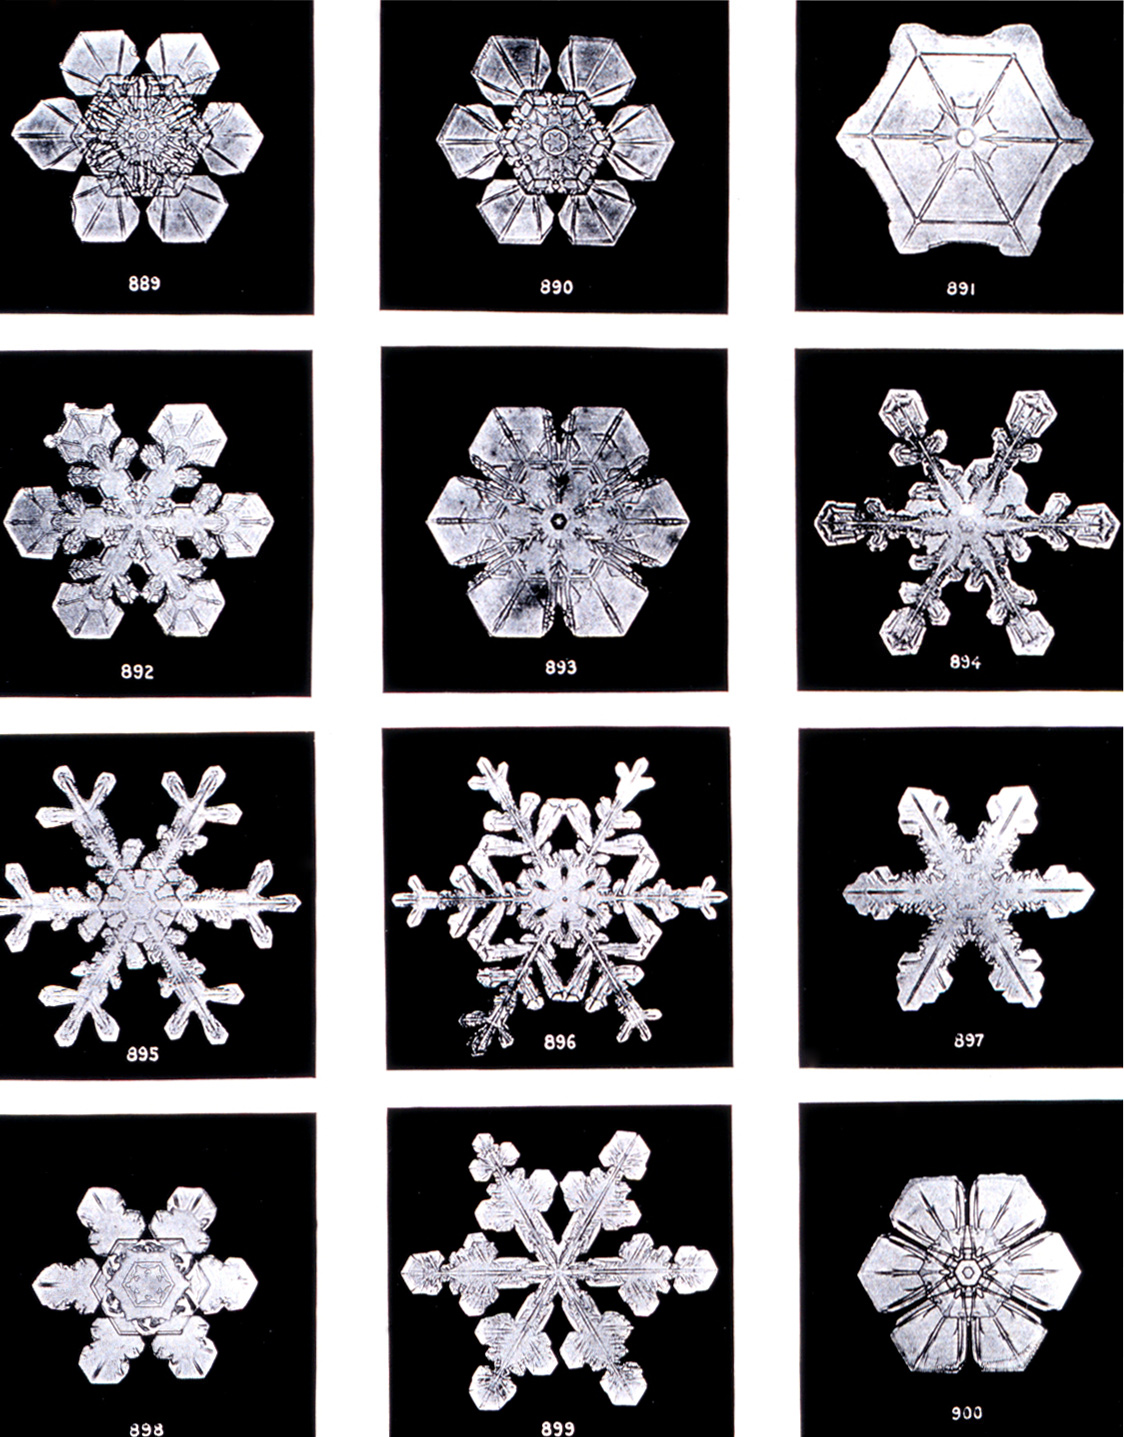
\includegraphics[width=0.4\linewidth]{images/book4/bentley-snowflakes.jpg}\hspace{1em}%
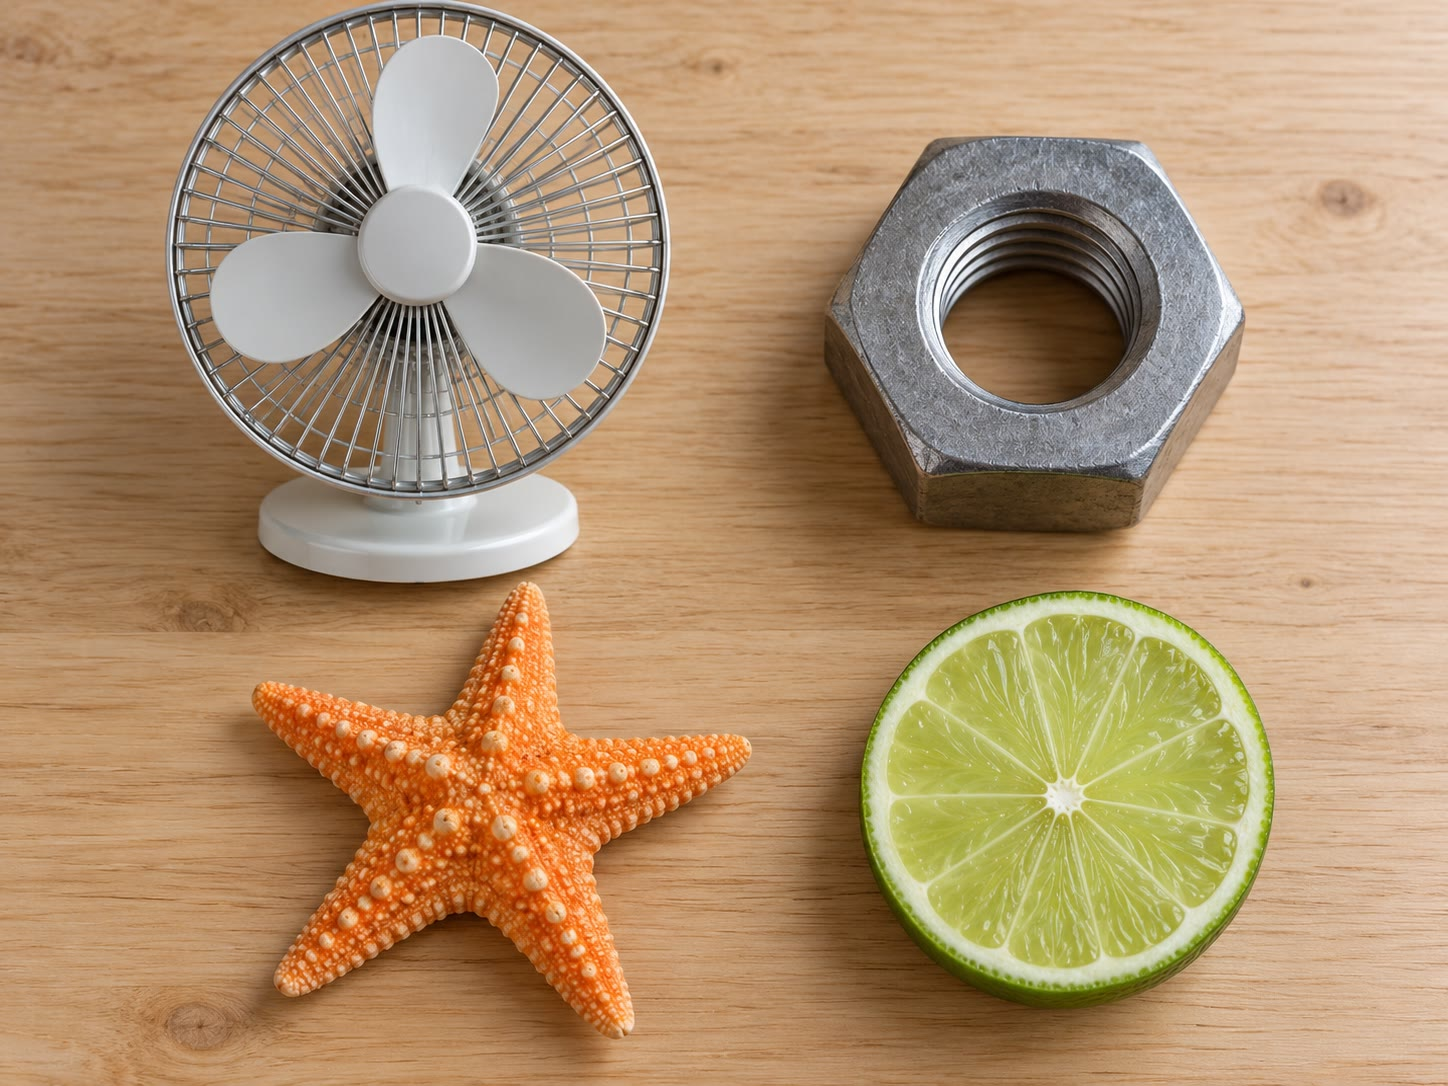
\includegraphics[width=0.48\linewidth]{images/book4/ai/b3-04-symmetric-objects.jpg}

{\small Kiri: kristal-kristal salju yang dipotret Wilson Bentley sekitar tahun
1902, masing-masing dengan simetri lipat enam. Kanan: benda-benda sehari-hari
dengan simetri rotasi lipat tiga, lipat enam, dan lipat lima.}
\end{omfigure}

\section{Operasi dan unsur simetri}

\begin{definition}[Operasi simetri, unsur simetri]\label{def:b3:point-groups:operation}
Yang disebut \emph{operasi simetri}\index{operasi simetri} adalah gerakan
atau pencerminan yang membawa sebuah molekul ke konfigurasi yang tak
terbedakan dari konfigurasi semula (setiap atom berada pada posisi yang
sebelumnya ditempati atom sejenis). Yang disebut \emph{unsur
simetri}\index{unsur simetri} adalah objek geometris --- sebuah titik, garis,
atau bidang --- yang menjadi acuan operasi itu.
\end{definition}

Setiap molekul mempunyai operasi identitas $E$, yang tidak melakukan apa-apa.
Operasi-operasi lainnya terbagi menjadi empat jenis.

\begin{definition}[Sumbu rotasi sejati, sumbu utama]\label{def:b3:point-groups:rotation}
Yang disebut \emph{sumbu rotasi sejati}\index{sumbu rotasi sejati} $C_n$
adalah garis yang rotasi sebesar $2\pi/n$ terhadapnya merupakan \omterm{def:b3:point-groups:operation}{operasi
simetri}, yang juga ditulis $C_n$; pangkat-pangkatnya $C_n^k$ adalah rotasi
sebesar $2\pi k/n$, dan $C_n^n = E$. Sumbu dengan $n$ tertinggi adalah
\emph{sumbu utama}\index{sumbu utama}, yang diambil sebagai $z$.
\end{definition}

\begin{definition}[Bidang cermin]\label{def:b3:point-groups:mirror}
Yang disebut \emph{bidang cermin}\index{bidang cermin} $\sigma$ adalah bidang
yang pencerminan terhadapnya merupakan \omterm{def:b3:point-groups:operation}{operasi simetri}; $\sigma^2 = E$. Sebuah
bidang cermin disebut \emph{bidang cermin
vertikal}\index{bidang cermin vertikal} $\sigma_v$ jika memuat \omterm{def:b3:point-groups:rotation}{sumbu utama}, \emph{bidang cermin
horizontal}\index{bidang cermin horizontal} $\sigma_h$ jika tegak lurus pada
sumbu itu, dan \emph{bidang cermin dihedral}\index{bidang cermin dihedral}
$\sigma_d$ jika memuat \omterm{def:b3:point-groups:rotation}{sumbu utama} dan membagi dua sudut antara dua sumbu
$C_2$ yang tegak lurus padanya.
\end{definition}

\begin{definition}[Pusat inversi]\label{def:b3:point-groups:inversion}
Yang disebut \emph{pusat inversi}\index{pusat inversi} $i$ adalah titik yang
inversi terhadapnya, $(x, y, z) \mapsto (-x, -y, -z)$, merupakan \omterm{def:b3:point-groups:operation}{operasi
simetri}.
\end{definition}

\begin{definition}[Sumbu rotasi tak sejati]\label{def:b3:point-groups:improper}
Yang disebut \emph{sumbu rotasi tak sejati}\index{sumbu rotasi tak sejati}
$S_n$ adalah garis yang rotasi sebesar $2\pi/n$ terhadapnya, diikuti
pencerminan pada bidang yang tegak lurus padanya, merupakan \omterm{def:b3:point-groups:operation}{operasi simetri}.
$S_1 = \sigma$ dan $S_2 = i$.
\end{definition}

\begin{example}[Unsur-unsur simetri empat molekul]\label{ex:b3:point-groups:elements}
\ce{H2O}: $E$, sumbu $C_2$ yang membagi dua sudut H--O--H, dan dua bidang
vertikal, yaitu bidang molekul dan bidang yang tegak lurus padanya. \ce{NH3}:
$E$, sebuah $C_3$ melalui N (operasi $C_3$ dan $C_3^2$), dan tiga $\sigma_v$,
masing-masing memuat satu ikatan N--H. \ce{BF3}: sebuah $C_3$, tiga $C_2$
sepanjang ikatan B--F, $\sigma_h$ (bidang molekul), tiga $\sigma_v$, dan sebuah
$S_3$. \ce{CH4}: empat $C_3$ sepanjang ikatan C--H, tiga $C_2$ yang membagi dua
sudut H--C--H, yang sekaligus merupakan sumbu $S_4$, dan enam $\sigma_d$,
masing-masing memuat dua ikatan C--H (gambar di bawah).
\end{example}

\begin{omfigure}
\begin{tikzpicture}[font=\small]
  % H2O, side view: molecular plane xz (shaded), C2 along z
  \begin{scope}
    \fill[omDef!10] (-1.5,-1.0) -- (1.5,-1.0) -- (1.5,1.2) -- (-1.5,1.2) -- cycle;
    \fill[omThm!12, opacity=0.8] (-0.45,-1.35) -- (0.45,-0.65) -- (0.45,1.55) -- (-0.45,0.85) -- cycle;
    \draw[densely dashed, black!70] (0,-1.4) -- (0,1.7) node[above] {$C_2$};
    \node[aO] (o) at (0,0.5) {};
    \node[aH] (h1) at (-0.95,-0.25) {};
    \node[aH] (h2) at (0.95,-0.25) {};
    \begin{scope}[on background layer]
      \draw[bond] (o.center) -- (h1.center) (o.center) -- (h2.center);
    \end{scope}
    \node[omDef, anchor=north west] at (-1.5,1.2) {$\sigma_v(xz)$};
    \node[omThm, anchor=west] at (0.5,-0.85) {$\sigma_v'(yz)$};
    \node[anchor=north] at (0,-1.6) {\ce{H2O}, $C_{2v}$};
  \end{scope}
  % NH3, top view along C3
  \begin{scope}[xshift=4.0cm]
    \foreach \a in {90,210,330}{\draw[ommirror] (0,0) -- (\a:1.35); \draw[ommirror, black!40] (0,0) -- (\a+180:1.0);}
    \foreach \a in {90,210,330}{\node[aH] at (\a:0.95) {};}
    \node[aN] at (0,0) {};
    \pic at (0,0) {omthreefold};
    \node[anchor=north] at (0,-1.6) {\ce{NH3}, $C_{3v}$ (dari atas)};
  \end{scope}
  % BF3, top view; sigma_h = plane of the paper (thick circle)
  \begin{scope}[xshift=8.0cm]
    \draw[ommirror] (0,0) circle (1.3);
    \foreach \a in {90,210,330}{\draw[ommirror] (\a:1.3) -- (\a+180:1.3);}
    \foreach \a in {90,210,330}{\pic[rotate=\a-90] at (\a:1.42) {omtwofold}; \pic[rotate=\a-90] at (\a+180:1.42) {omtwofold};}
    \foreach \a in {90,210,330}{\node[aF] at (\a:0.95) {};}
    \node[aX={pink!70!gray}{5.6mm}] at (0,0) {};
    \pic at (0,0) {omthreefold};
    \node[anchor=north] at (0,-1.6) {\ce{BF3}, $D_{3h}$ (dari atas)};
  \end{scope}
\end{tikzpicture}

{\small \omterm{def:b3:point-groups:operation}{Unsur-unsur simetri}. \ce{H2O}: sumbu $C_2$ (garis putus-putus) dan dua
\omterm{def:b3:point-groups:mirror}{bidang cermin vertikal}. \ce{NH3} dan \ce{BF3} dilihat sepanjang \omterm{def:b3:point-groups:rotation}{sumbu utamanya}
(lambang segitiga): garis tebal adalah \omterm{def:b3:point-groups:mirror}{bidang cermin} yang terlihat dari
sisinya; pada \ce{BF3} lingkaran tebal menandai \omterm{def:b3:point-groups:mirror}{bidang cermin horizontal}
(bidang halaman) dan lambang lensa menandai ketiga sumbu $C_2$ yang terletak
di dalamnya.}
\end{omfigure}

\section{Grup}

\begin{proposition}[Hasil kali operasi simetri]\label{prop:b3:point-groups:closure}
Melakukan dua \omterm{def:b3:point-groups:operation}{operasi simetri} sebuah molekul berturut-turut menghasilkan lagi
sebuah \omterm{def:b3:point-groups:operation}{operasi simetri} molekul itu. Bersama $E$ dan invers setiap operasi,
himpunan \omterm{def:b3:point-groups:operation}{operasi simetri} membentuk sebuah grup: hasil kali yang asosiatif,
sebuah identitas, dan invers untuk setiap unsur.
\end{proposition}

\begin{proof}
Setiap operasi membuat molekul tak terbedakan dari dirinya sendiri, sehingga
dua operasi berturut-turut juga demikian. Hasil kali operasi (komposisi
pemetaan ruang) bersifat asosiatif; $E$ adalah identitasnya; operasi yang
dibatalkan (rotasi dengan sudut berlawanan, pencerminan yang diulang) juga
merupakan \omterm{def:b3:point-groups:operation}{operasi simetri}.
\end{proof}

\begin{proposition}[Sebuah titik bersama]\label{prop:b3:point-groups:fixed-point}
Semua \omterm{def:b3:point-groups:operation}{unsur simetri} sebuah molekul berhingga melalui satu titik.
\end{proposition}

\begin{proof}
Setiap \omterm{def:b3:point-groups:operation}{operasi simetri} memetakan setiap atom ke atom yang bermassa sama,
sehingga operasi itu tidak mengubah pusat massa. Rotasi hanya membiarkan
tetap titik-titik pada sumbunya, pencerminan titik-titik pada bidangnya, dan
rotasi tak sejati atau inversi hanya satu titik: setiap unsur memuat pusat
massa.
\end{proof}

\begin{definition}[Grup titik, orde grup titik]\label{def:b3:point-groups:point-group}
Grup semua \omterm{def:b3:point-groups:operation}{operasi simetri} sebuah molekul disebut \emph{grup
titik}\index{grup titik} molekul itu, dinamai demikian karena satu titik tetap
diam. Banyaknya operasi grup itu disebut \emph{orde grup
titik}\index{orde grup titik}, $h$.
\end{definition}

\begin{example}[Grup air]\label{ex:b3:point-groups:c2v}
Keempat operasi $E$, $C_2$, $\sigma_v(xz)$, $\sigma_v'(yz)$ dari \ce{H2O}
membentuk grup berorde 4. Tabel perkaliannya (operasi baris dilakukan
sesudah operasi kolom) adalah
\begin{center}\small
\begin{tabular}{c|cccc}
\hline
 & $E$ & $C_2$ & $\sigma_v(xz)$ & $\sigma_v'(yz)$\\ \hline
$E$ & $E$ & $C_2$ & $\sigma_v(xz)$ & $\sigma_v'(yz)$\\
$C_2$ & $C_2$ & $E$ & $\sigma_v'(yz)$ & $\sigma_v(xz)$\\
$\sigma_v(xz)$ & $\sigma_v(xz)$ & $\sigma_v'(yz)$ & $E$ & $C_2$\\
$\sigma_v'(yz)$ & $\sigma_v'(yz)$ & $\sigma_v(xz)$ & $C_2$ & $E$\\ \hline
\end{tabular}
\end{center}
Misalnya, titik $(x, y, z)$ yang dicerminkan terhadap $xz$ pindah ke
$(x, -y, z)$, lalu diputar sebesar $\pi$ terhadap $z$ ke $(-x, y, z)$: sama
dengan satu pencerminan terhadap $yz$.
\end{example}

\begin{definition}[Kelas operasi simetri, subgrup]\label{def:b3:point-groups:class}
Dua operasi $A$ dan $B$ termasuk dalam \emph{kelas operasi
simetri}\index{kelas operasi simetri} yang sama jika $B = X^{-1}AX$ untuk suatu
operasi $X$ dalam grup itu: keduanya adalah operasi sejenis, yang dilihat
dalam kerangka yang dipindahkan oleh $X$. Himpunan bagian sebuah grup yang
merupakan grup tersendiri disebut \emph{subgrup}\index{subgrup}; ordenya
membagi orde grup.
\end{definition}

\begin{example}[Kelas-kelas \ce{NH3}]\label{ex:b3:point-groups:classes}
Dalam $C_{3v}$ ($h = 6$), ketiga pencerminan membentuk satu kelas (rotasi
$C_3$ membawa setiap bidang ke bidang lain), kedua rotasi $C_3$ dan $C_3^2$
kelas yang lain, dan $E$ satu kelas tersendiri: tiga kelas, ditulis $E$,
$2C_3$, $3\sigma_v$. Dalam $C_{2v}$ setiap operasi merupakan kelasnya sendiri:
tidak ada operasi yang mengubah bidang yang satu menjadi bidang yang lain.
\end{example}

\begin{definition}[Simbol Schoenflies]\label{def:b3:point-groups:schoenflies}
Sebuah \omterm{def:b3:point-groups:point-group}{grup titik} dinamai dengan \emph{simbol Schoenflies}\index{simbol Schoenflies}:
$C_n$ (satu sumbu $C_n$), $C_{nv}$ (ditambah $n$ bidang vertikal), $C_{nh}$
(ditambah $\sigma_h$), $D_n$ (ditambah $n$ sumbu $C_2$ yang tegak lurus pada
$C_n$), $D_{nh}$ dan $D_{nd}$ ($\sigma_h$, atau $n$ bidang dihedral,
ditambahkan pada $D_n$), $S_{2n}$, grup-grup kubik $T_d$, $O_h$, $I_h$ untuk
tetrahedron, oktahedron, dan ikosahedron, serta $C_s$, $C_i$, $C_1$ untuk
molekul yang hanya mempunyai satu \omterm{def:b3:point-groups:mirror}{bidang cermin}, hanya satu \omterm{def:b3:point-groups:inversion}{pusat inversi},
atau tidak mempunyai apa pun. Molekul linear termasuk dalam $C_{\infty v}$
atau $D_{\infty h}$.
\end{definition}

\section{Menentukan grup titik}

\begin{method}[Mencari grup titik sebuah molekul]\label{met:b3:point-groups:assign}
\begin{enumerate}
  \item Apakah molekulnya linear? Dengan \omterm{def:b3:point-groups:inversion}{pusat inversi}, $D_{\infty h}$
        (\ce{CO2}, \ce{N2}); tanpa \omterm{def:b3:point-groups:inversion}{pusat inversi}, $C_{\infty v}$ (\ce{HCl}, \ce{HCN}).
  \item Apakah molekulnya mempunyai beberapa sumbu berorde tinggi
        ($n \ge 3$)? Bentuk tetrahedral: $T_d$; oktahedral: $O_h$;
        ikosahedral: $I_h$.
  \item Carilah \omterm{def:b3:point-groups:rotation}{sumbu utama} $C_n$ (jika tidak ada: $C_s$ jika ada bidang,
        $C_i$ jika ada pusat, dan $C_1$ jika tidak ada keduanya).
  \item Apakah ada $n$ sumbu $C_2$ yang tegak lurus pada $C_n$? Jika ya,
        grupnya adalah $D_{nh}$ (dengan $\sigma_h$), atau $D_{nd}$ (dengan $n$
        $\sigma_d$), atau $D_n$.
  \item Jika tidak: $C_{nh}$ (dengan $\sigma_h$), $C_{nv}$ (dengan $n$
        $\sigma_v$), $S_{2n}$ (hanya dengan sebuah $S_{2n}$ yang segaris
        dengan $C_n$), atau $C_n$.
\end{enumerate}
\end{method}

\begin{omfigure}
\begin{tikzpicture}[font=\footnotesize, node distance=6mm and 11mm,
  q/.style={draw=black!60, fill=omDef!6, rounded corners=2pt, align=center, inner sep=3pt},
  g/.style={draw=black!60, fill=omProp!10, rounded corners=2pt, inner sep=3pt}]
  \node[q] (lin) {linear?};
  \node[g, right=of lin] (dinf) {$D_{\infty h}$ / $C_{\infty v}$ (dengan / tanpa $i$)};
  \node[q, below=of lin] (cub) {dua $C_n$ atau lebih, $n \ge 3$?};
  \node[g, right=of cub] (td) {$T_d$, $O_h$, $I_h$};
  \node[q, below=of cub] (cn) {ada sumbu $C_n$?};
  \node[g, right=of cn] (low) {$C_s$, $C_i$ atau $C_1$ (tidak)};
  \node[q, below=of cn] (c2) {$n$ $C_2 \perp C_n$?};
  \node[q, right=of c2, xshift=6mm] (dh) {$\sigma_h$?\; jika tidak, $n$ $\sigma_d$?};
  \node[g, right=of dh] (dg) {$D_{nh}$ / $D_{nd}$ / $D_n$};
  \node[q, below=of c2] (sh) {$\sigma_h$?\; jika tidak, $n$ $\sigma_v$?\; jika tidak, $S_{2n}$?};
  \node[g, right=of sh] (cg) {$C_{nh}$ / $C_{nv}$ / $S_{2n}$ / $C_n$};
  \draw[->] (lin) -- node[above] {ya} (dinf);
  \draw[->] (lin) -- node[left] {tidak} (cub);
  \draw[->] (cub) -- node[above] {ya} (td);
  \draw[->] (cub) -- node[left] {tidak} (cn);
  \draw[->] (cn) -- node[above] {tidak} (low);
  \draw[->] (cn) -- node[left] {ya} (c2);
  \draw[->] (c2) -- node[above] {ya} (dh);
  \draw[->] (dh) -- (dg);
  \draw[->] (c2) -- node[left] {tidak} (sh);
  \draw[->] (sh) -- (cg);
\end{tikzpicture}

{\small Pencarian \omterm{def:b3:point-groups:point-group}{grup titik}, dalam urutan metode di atas.}
\end{omfigure}

\begin{example}[Sebuah galeri]\label{ex:b3:point-groups:gallery}
\ce{H2O}, \ce{CH2Cl2}, \ce{SO2}: $C_{2v}$. \ce{NH3}, \ce{CHCl3}: $C_{3v}$. \ce{BF3},
\ce{PCl5}: $D_{3h}$. \ce{CH4}, \ce{CCl4}: $T_d$. \ce{SF6}: $O_h$. Benzena: $D_{6h}$.
Etena: $D_{2h}$. Etana: $D_{3d}$ jika bersilang, $D_{3h}$ jika eklips. Alena
\ce{H2C=C=CH2}: $D_{2d}$, kedua bidang \ce{CH2} saling tegak lurus.
Sikloheksana dalam konformasi kursi: $D_{3d}$. trans-\ce{N2F2}: $C_{2h}$.
\ce{CHFClBr}: $C_1$.
\end{example}

\begin{omfigure}
\tdplotsetmaincoords{60}{100}
\begin{tikzpicture}[tdplot_main_coords, scale=1.6, font=\small]
  \pic[transform shape] {omcubeo={2}};
  % depth order for view 60/100 (smallest first): H(0,0,0), H(0,2,2), C, H(2,2,0), H(2,0,2)
  \draw[densely dashed, omThm, thick] (-0.4,-0.4,-0.4) -- (2.5,2.5,2.5) node[anchor=south west] {$C_3$};
  \draw[densely dashed, omDef, thick] (1,1,-0.5) -- (1,1,2.6) node[anchor=south] {$S_4$, $C_2$};
  \node[aH] (h1) at (0,0,0) {};
  \node[aH] (h4) at (0,2,2) {};
  \node[aC] (c) at (1,1,1) {};
  \node[aH] (h2) at (2,2,0) {};
  \node[aH] (h3) at (2,0,2) {};
  \begin{scope}[on background layer]
    \draw[bond] (c.center) -- (h1.center) (c.center) -- (h2.center)
                (c.center) -- (h3.center) (c.center) -- (h4.center);
  \end{scope}
\end{tikzpicture}

{\small Metana dalam sebuah kubus, dengan karbon di pusat dan hidrogen-hidrogennya
pada sudut-sudut yang berselang-seling. Diagonal ruang yang melalui satu
hidrogen adalah sumbu $C_3$ (ada empat); sumbu yang melalui pusat dua sisi
yang berhadapan adalah sumbu $C_2$ sekaligus $S_4$ (ada tiga). \omterm{def:b3:point-groups:point-group}{Grup titiknya}
$T_d$, berorde 24.}
\end{omfigure}

\section{Akibat-akibatnya: kepolaran dan kiralitas}

\begin{theorem}[Molekul polar]\label{thm:b3:point-groups:polar}
Sebuah molekul hanya dapat mempunyai momen dipol permanen jika \omterm{def:b3:point-groups:point-group}{grup titiknya}
$C_1$, $C_s$, $C_n$ atau $C_{nv}$; dipol itu kemudian terletak sepanjang
\omterm{def:b3:point-groups:rotation}{sumbu utama} (pada bidangnya, untuk $C_s$).
\end{theorem}

\begin{proof}
Momen dipol adalah sifat vektor molekul, sehingga setiap \omterm{def:b3:point-groups:operation}{operasi simetri}
harus membiarkannya tidak berubah. Rotasi terhadap suatu sumbu hanya
membiarkan tetap vektor-vektor sepanjang sumbu itu; dua sumbu tidak
membiarkan tetap vektor tak nol mana pun; $\sigma_h$, $i$ atau $S_n$ membalik
setiap vektor sepanjang sumbu; $\sigma_v$ membiarkan tetap vektor-vektor pada
bidangnya. Jadi, dipol tak nol mensyaratkan paling banyak satu sumbu, tanpa
$\sigma_h$, tanpa $i$, tanpa $S_n$: grup-grup yang telah disebutkan.
\end{proof}

\begin{example}[Polar atau tidak]\label{ex:b3:point-groups:polar}
\ce{H2O}, \ce{NH3}, \ce{CHCl3} dan \ce{SO2} ($C_{2v}$, $C_{3v}$) dapat bersifat
polar, dan memang polar. \ce{BF3} ($D_{3h}$), \ce{CO2} ($D_{\infty h}$), \ce{CH4}
($T_d$), \ce{SF6} ($O_h$) dan trans-\ce{N2F2} ($C_{2h}$) tidak dapat polar,
bagaimanapun polarnya ikatan-ikatannya.
\end{example}

\begin{theorem}[Molekul kiral]\label{thm:b3:point-groups:chiral}
Sebuah molekul kiral jika dan hanya jika molekul itu tidak mempunyai \omterm{def:b3:point-groups:improper}{sumbu
rotasi tak sejati} $S_n$ (termasuk $S_1 = \sigma$ dan $S_2 = i$).
\end{theorem}

\begin{proof}
Jika molekul itu mempunyai sebuah $S_n$, maka $S_n = \sigma_hC_n$: bayangan
cermin $\sigma_h$ molekul itu sama dengan $C_n^{-1}$ yang dikenakan pada
molekul setelah $S_n$, yaitu molekul yang diputar --- dapat ditumpangtindihkan,
sehingga akiral. Sebaliknya, jika molekul itu akiral, bayangan cerminnya
$\sigma M$ dapat dibawa ke $M$ oleh gerakan sejati $R$ (rotasi terhadap pusat
massa): $R\sigma$ lalu merupakan \omterm{def:b3:point-groups:operation}{operasi simetri}. Operasi itu tak sejati
(operasi itu mengubah tangan kiri menjadi tangan kanan, dan matriksnya
berdeterminan $-1$), dan
setiap operasi tak sejati dalam \omterm{def:b3:point-groups:point-group}{grup titik} adalah sebuah $S_n$ untuk suatu
$n$ (rotasi yang diikuti pencerminan pada bidang yang tegak lurus). Jadi
molekul itu mempunyai sebuah $S_n$.
\end{proof}

\begin{example}[Molekul akiral tanpa bidang]\label{ex:b3:point-groups:s4}
Ada molekul yang tidak mempunyai \omterm{def:b3:point-groups:mirror}{bidang cermin} maupun \omterm{def:b3:point-groups:inversion}{pusat inversi}, tetapi
akiral karena sebuah sumbu $S_4$: contoh klasiknya adalah senyawa spiro yang
tersusun dari dua cincin bersubstituen identik yang saling tegak lurus,
dengan \omterm{def:b3:point-groups:point-group}{grup titik} $S_4$. Kiralitas tidak dapat dinilai hanya dengan mencari
sebuah bidang.
\end{example}

\section{Representasi dan tabel karakter}

Setiap \omterm{def:b3:point-groups:operation}{operasi simetri} memindahkan sebuah titik $(x, y, z)$ secara linear:
operasi itu dapat ditulis sebagai matriks $3\times3$.

\begin{definition}[Representasi matriks, karakter]\label{def:b3:point-groups:representation}
Yang disebut \emph{representasi matriks}\index{representasi matriks} $\Gamma$
sebuah \omterm{def:b3:point-groups:point-group}{grup titik} adalah aturan yang memadankan setiap operasi $R$ dengan
matriks persegi $D(R)$ sedemikian sehingga $D(R_1R_2) = D(R_1)D(R_2)$: hasil
kali operasi menjadi hasil kali matriks. Yang disebut
\emph{karakter}\index{karakter} $\chi(R)$ dari $R$ dalam $\Gamma$ adalah jejak (\textit{trace})
$D(R)$.
\end{definition}

\begin{example}[Koordinat-koordinat dalam $C_{3v}$]\label{ex:b3:point-groups:xyz}
Untuk $C_3$ terhadap $z$, $D = \begin{psmallmatrix}\cos120^\circ & -\sin120^\circ &
0\\ \sin120^\circ & \cos120^\circ & 0\\ 0 & 0 & 1\end{psmallmatrix}$, dengan
jejak $2\cos120^\circ + 1 = 0$; untuk $\sigma_v(xz)$,
$D = \mathrm{diag}(1, -1, 1)$, dengan jejak 1; untuk $E$, jejak 3.
\omterm{def:b3:point-groups:representation}{Karakter-karakter} representasi ini adalah $(3, 0, 1)$ pada kelas-kelas
$(E, 2C_3, 3\sigma_v)$. Setiap matriks berbentuk diagonal blok, dengan blok
$2\times2$ untuk $(x, y)$ dan blok $1\times1$ untuk $z$: representasi itu
terpecah menjadi dua representasi yang lebih kecil.
\end{example}

\begin{proposition}[Karakter adalah fungsi kelas]\label{prop:b3:point-groups:class-characters}
Operasi-operasi dalam kelas yang sama mempunyai \omterm{def:b3:point-groups:representation}{karakter} yang sama dalam
representasi mana pun.
\end{proposition}

\begin{proof}
Jika $B = X^{-1}AX$, maka $D(B) = D(X)^{-1}D(A)D(X)$, dan jejak tidak berubah
oleh perubahan basis semacam itu: $\mathrm{tr}(P^{-1}MP) = \mathrm{tr}(M)$.
\end{proof}

\begin{proposition}[Mereduksi menurut blok]\label{prop:b3:point-groups:direct-sum}
Jika sebuah basis dapat dipecah menjadi himpunan-himpunan bagian yang
masing-masing dipetakan ke dirinya sendiri oleh setiap operasi, maka semua
matriksnya berbentuk diagonal blok, dan representasinya adalah jumlah
representasi-representasi yang lebih kecil yang dibawa oleh
himpunan-himpunan bagian itu; \omterm{def:b3:point-groups:representation}{karakternya} adalah jumlah \omterm{def:b3:point-groups:representation}{karakter} mereka.
\end{proposition}

\begin{proof}
Operasi yang memetakan setiap himpunan bagian ke dirinya sendiri tidak
mempunyai unsur matriks di antara himpunan bagian yang berbeda; jejak matriks
diagonal blok adalah jumlah jejak blok-bloknya.
\end{proof}

\begin{definition}[Representasi tak tereduksi, tabel karakter, simbol Mulliken]\label{def:b3:point-groups:irrep}
Representasi yang tidak dapat dipecah lebih lanjut oleh perubahan basis apa
pun disebut \emph{representasi tak
tereduksi}\index{representasi tak tereduksi}. Yang disebut \emph{tabel karakter}\index{tabel karakter} sebuah
\omterm{def:b3:point-groups:point-group}{grup titik} adalah daftar \omterm{def:b3:point-groups:representation}{karakter} representasi-representasi tak tereduksinya,
satu baris untuk setiap representasi, pada kelas-kelasnya, satu kolom untuk
setiap kelas, beserta fungsi Kartesius dan rotasi yang bertransformasi
seperti setiap baris. Baris-baris itu dinamai dengan \emph{simbol
Mulliken}\index{simbol Mulliken}: $A$ atau $B$ untuk satu dimensi (simetris
atau antisimetris terhadap rotasi utama), $E$ untuk dua, $T$ untuk tiga;
subskrip 1, 2 (simetris atau antisimetris terhadap $C_2$ atau $\sigma_v$),
$g$, $u$ (terhadap inversi), aksen (terhadap $\sigma_h$).
\end{definition}

\begin{proposition}[Ukuran tabel karakter]\label{prop:b3:point-groups:irrep-count}
Sebuah \omterm{def:b3:point-groups:point-group}{grup titik} mempunyai \omterm{def:b3:point-groups:irrep}{representasi tak tereduksi} sebanyak kelasnya, dan
jumlah kuadrat dimensi-dimensinya sama dengan ordenya: $\sum_id_i^2 = h$.
\end{proposition}
\begin{proof}[Kedudukan pernyataan ini]
Dibuktikan dalam \cref{ch:b3:group-theory-applied} dari keortogonalan
\omterm{def:b3:point-groups:representation}{karakter}, yang di sana sendiri diterima tanpa bukti.
\end{proof}

% ledger: ct:C2v, ct:C3v, ct:Td
Tabel-tabel yang paling sering diperlukan dalam buku ini adalah tabel untuk
air, amonia, dan metana:
\begin{omchartable}{C_{2v}}{cccc}{E & C_2 & \sigma_v(xz) & \sigma_v'(yz)}
A_1 & 1 & 1 & 1 & 1 & z & x^2,\ y^2,\ z^2 \\
A_2 & 1 & 1 & -1 & -1 & R_z & xy \\
B_1 & 1 & -1 & 1 & -1 & x,\ R_y & xz \\
B_2 & 1 & -1 & -1 & 1 & y,\ R_x & yz \\
\end{omchartable}
\begin{omchartable}{C_{3v}}{ccc}{E & 2C_3 & 3\sigma_v}
A_1 & 1 & 1 & 1 & z & x^2 + y^2,\ z^2 \\
A_2 & 1 & 1 & -1 & R_z & \\
E & 2 & -1 & 0 & (x, y),\ (R_x, R_y) & (x^2 - y^2, xy),\ (xz, yz) \\
\end{omchartable}
\begin{omchartable}{T_d}{ccccc}{E & 8C_3 & 3C_2 & 6S_4 & 6\sigma_d}
A_1 & 1 & 1 & 1 & 1 & 1 & & x^2 + y^2 + z^2 \\
A_2 & 1 & 1 & 1 & -1 & -1 & & \\
E & 2 & -1 & 2 & 0 & 0 & & (2z^2 - x^2 - y^2,\ x^2 - y^2) \\
T_1 & 3 & 0 & -1 & 1 & -1 & (R_x, R_y, R_z) & \\
T_2 & 3 & 0 & -1 & -1 & 1 & (x, y, z) & (xy, xz, yz) \\
\end{omchartable}

\begin{method}[Membaca tabel karakter]\label{met:b3:point-groups:matrices}
\begin{enumerate}
  \item Kolom \omterm{def:b3:point-groups:representation}{karakter} pertama (di bawah $E$) adalah dimensinya: \omterm{def:b3:quantum-model-systems:degenerate}{degenerasi}
        tingkat-tingkat atau orbital-orbital yang ditandai dengan baris itu.
  \item \omterm{def:b3:point-groups:representation}{Karakter} $+1$ berarti fungsi itu tidak berubah oleh operasinya, $-1$
        berarti fungsi itu berganti tanda; 0 pada baris terdegenerasi berarti
        anggota-anggota himpunannya bercampur.
  \item Untuk mengetahui cara sebuah fungsi bertransformasi, kenakan setiap
        operasi padanya dan bandingkan dengan baris-barisnya; kolom-kolom di
        sebelah kanan memberikan jawabannya untuk $x$, $y$, $z$, rotasi, dan
        fungsi-fungsi kuadratik (bentuk orbital $d$).
\end{enumerate}
\end{method}

\begin{example}[Orbital-orbital oksigen dalam air]\label{ex:b3:point-groups:water-orbitals}
Dalam $C_{2v}$, orbital $2s$ dan $2p_z$ oksigen tidak berubah oleh setiap
operasi: $a_1$ (huruf kecil untuk orbital). $2p_x$ berganti tanda oleh $C_2$
dan $\sigma_v'(yz)$: $b_1$. $2p_y$: $b_2$. Inilah label-label yang dipakai untuk
orbital air dalam jilid Tahun 2; \cref{ch:b3:group-theory-applied}
menurunkan label kombinasi-kombinasi hidrogen.
\end{example}

\begin{omfigure}
\begin{tikzpicture}[font=\small]
  \begin{scope}
    \pic {omstereo={1.2}};
    \draw[ommirror] (-1.2,0) -- (1.2,0);
    \draw[ommirror] (0,-1.2) -- (0,1.2);
    \pic at (0,0) {omtwofold};
    \foreach \x/\y in {0.55/0.45,-0.55/0.45,0.55/-0.45,-0.55/-0.45}{\pic at (\x,\y) {omup};}
    \node[anchor=north] at (0,-1.35) {$C_{2v}$};
  \end{scope}
  \begin{scope}[xshift=4cm]
    \pic {omstereo={1.2}};
    \foreach \a in {90,210,330}{\draw[ommirror] (\a:1.2) -- (\a+180:1.2);}
    \pic at (0,0) {omthreefold};
    \foreach \a in {70,110,190,230,310,350}{\pic at (\a:0.75) {omup};}
    \node[anchor=north] at (0,-1.35) {$C_{3v}$};
  \end{scope}
  \begin{scope}[xshift=8cm]
    \pic {omstereo={1.2}};
    \draw[ommirror] (0,0) circle (1.2);
    \foreach \a in {90,210,330}{\draw[ommirror] (\a:1.2) -- (\a+180:1.2);}
    \pic at (0,0) {omthreefold};
    \foreach \a in {70,110,190,230,310,350}{\pic at (\a:0.75) {omup}; \pic at (\a:0.75) {omdown};}
    \node[anchor=north] at (0,-1.35) {$D_{3h}$};
  \end{scope}
\end{tikzpicture}

{\small Proyeksi stereografik. Sebuah titik umum di atas bidang ekuator
(noktah) dibawa oleh operasi-operasi grup ke semua titik yang diperlihatkan;
tanda silang menandai titik di bawah bidang itu. Garis dan lingkaran tebal:
\omterm{def:b3:point-groups:mirror}{bidang cermin}. $C_{2v}$: 4 titik; $C_{3v}$: 6; $D_{3h}$: 12 (6 di atas, 6 di
bawah, saling bertumpuk): banyaknya titik sama dengan orde grup.}
\end{omfigure}

\begin{history}[Schoenflies dan simetri kristal]
Arthur Schoenflies, seorang matematikawan, pada tahun 1891 mengelompokkan
230 grup ruang kristal; ke-32 \omterm{def:b3:point-groups:point-group}{grup titik} kristalografis yang dinamainya
masih ditulis dengan simbol-simbolnya. Para kimiawan mengambil notasi itu
pada tahun 1930-an, ketika teori grup mulai diterapkan pada spektrum
molekul.
\end{history}

\begin{inthelab}[Simetri dengan kit model]
Cara tercepat untuk menemukan \omterm{def:b3:point-groups:operation}{unsur-unsur simetri} sebuah molekul yang belum
dikenal adalah merakitnya dengan kit model molekul dan memutarnya di tangan,
sambil mencari sumbu yang membuat molekul itu tampak sama setelah diputar
sebagian, dan bidang yang membelahnya menjadi dua bagian yang saling bayangan
cermin. Program komputasi juga melaporkan \omterm{def:b3:point-groups:point-group}{grup titik} sebuah struktur yang
telah dioptimasi, dalam suatu toleransi.
\end{inthelab}

\section{Latihan}

\begin{exercise}[$\star$]\label{exo:b3:point-groups:1}
Daftarlah \omterm{def:b3:point-groups:operation}{unsur-unsur simetri} dan berikan \omterm{def:b3:point-groups:point-group}{grup titik} dari: etena, \ce{XeF4},
\ce{PCl5}, 1,3,5-triklorobenzena.
\end{exercise}

\begin{exercise}[$\star$]\label{exo:b3:point-groups:2}
Berikan \omterm{def:b3:point-groups:point-group}{grup titik} etana bersilang dan etana eklips, serta \omterm{def:b3:point-groups:point-group}{grup titik}
sikloheksana dalam konformasi kursi.
\end{exercise}

\begin{exercise}[$\star$]\label{exo:b3:point-groups:3}
Manakah di antara molekul berikut yang dapat bersifat polar: \ce{SO3},
\ce{SO2}, \ce{PCl3}, \ce{XeF4}, \ce{CH2Cl2}, cis- dan trans-1,2-dikloroetena?
\end{exercise}

\begin{exercise}[$\star$]\label{exo:b3:point-groups:4}
Tuliskan matriks $3\times3$ untuk $C_2(z)$, $i$ dan $\sigma_h$ yang bekerja pada
$(x, y, z)$, beserta \omterm{def:b3:point-groups:representation}{karakternya}.
\end{exercise}

\begin{exercise}[$\star\star$]\label{exo:b3:point-groups:5}
Susunlah tabel perkalian $C_{2h}$, dengan operasi $E$, $C_2$, $i$, $\sigma_h$.
Apakah setiap operasi merupakan kelasnya sendiri?
\end{exercise}

\begin{exercise}[$\star\star$]\label{exo:b3:point-groups:6}
Dalam $C_{3v}$, hitunglah $\sigma_v(1)\,C_3$ dan $C_3\,\sigma_v(1)$ dengan
mengikuti sebuah titik. Apakah keduanya sama? Apa artinya bagi grup itu?
\end{exercise}

\begin{exercise}[$\star\star$]\label{exo:b3:point-groups:7}
Tunjukkan bahwa bifenil yang terpuntir dengan sudut antara 0 dan
90\textdegree\ di antara cincin-cincinnya termasuk dalam $D_2$, lalu
simpulkan kiralitasnya.
\end{exercise}

\begin{exercise}[$\star\star$]\label{exo:b3:point-groups:8}
Dengan memakai tabel $C_{2v}$, carilah label orbital-orbital $3d$ oksigen
dalam air (ambil fungsi-fungsi kuadratik sebagai bentuknya).
\end{exercise}

\begin{exercise}[$\star\star$]\label{exo:b3:point-groups:9}
Periksalah pada tabel $T_d$ bahwa $\sum_id_i^2 = h$ dan bahwa baris $A_1$
dan $T_2$ ortogonal jika setiap kolom diberi bobot sebesar ukuran kelasnya.
\end{exercise}

\begin{exercise}[$\star\star\star$]\label{exo:b3:point-groups:10}
Tunjukkan bahwa hasil kali dua pencerminan terhadap bidang-bidang yang
membentuk sudut $\theta$ adalah rotasi sebesar $2\theta$ terhadap garis
potong keduanya. Simpulkan bahwa molekul dengan dua bidang vertikal yang
membentuk sudut 60\textdegree\ mempunyai sumbu $C_3$.
\end{exercise}

\begin{exercise}[$\star\star\star$]\label{exo:b3:point-groups:11}
Alena \ce{H2C=C=CH2} mempunyai kedua gugus \ce{CH2} pada bidang-bidang yang
saling tegak lurus. Carilah \omterm{def:b3:point-groups:operation}{unsur-unsur simetrinya}, tunjukkan bahwa \omterm{def:b3:point-groups:point-group}{grup
titiknya} $D_{2d}$, dan jelaskan mengapa 1,3-dikloroalena \ce{ClHC=C=CHCl}
kiral.
\end{exercise}

\begin{exercise}[$\star\star\star$]\label{exo:b3:point-groups:12}
Bergerak dari \ce{SF6} ($O_h$) ke \ce{SF5Cl}, lalu ke trans-\ce{SF4Cl2} dan
cis-\ce{SF4Cl2}, berikan \omterm{def:b3:point-groups:point-group}{grup titik} masing-masing dan tunjukkan bahwa
masing-masing merupakan \omterm{def:b3:point-groups:class}{subgrup} dari $O_h$. Manakah yang dapat bersifat polar?
\end{exercise}

\section{Soal: Menyubstitusi Metana}

\begin{problem}[{Soal akhir pekan --- ke-24 operasi simetri metana, grup
titik turunan-turunan terklorinasinya, kepolaran dan kiralitas menurut
teorema, dan penghitungan isomer}]
\label{pb:b3:point-groups:1}
% ledger: ct:Td
Metana digambar dalam kubus bersisi 2 yang berpusat di titik asal, dengan
hidrogen-hidrogen pada sudut $(1,1,1)$, $(1,-1,-1)$, $(-1,1,-1)$ dan
$(-1,-1,1)$.

\medskip\noindent\textbf{Bagian I --- Grup metana.}
\begin{enumerate}[beginpenalty=10000]
  \item Carilah keempat sumbu $C_3$ dan hitunglah rotasi-rotasi yang
        diberikannya.
  \item Carilah ketiga sumbu $C_2$ dan periksalah bahwa masing-masing juga
        merupakan sumbu $S_4$; hitunglah operasi-operasi $S_4$.
  \item Carilah keenam \omterm{def:b3:point-groups:mirror}{bidang cermin} dan ikatan-ikatan C--H yang dimuat
        masing-masing.
  \item Tambahkan $E$: berapakah orde grupnya?
  \item Periksalah bahwa tidak ada \omterm{def:b3:point-groups:inversion}{pusat inversi}. (Apakah $(-1,-1,-1)$
        merupakan posisi sebuah hidrogen?)
  \item Kelompokkan operasi-operasi itu ke dalam kelima kelas tabel $T_d$.
\end{enumerate}

\medskip\noindent\textbf{Bagian II --- Metana-metana terklorinasi.}
\begin{enumerate}[resume, beginpenalty=10000]
  \item Berikan \omterm{def:b3:point-groups:point-group}{grup titik} \ce{CH3Cl} beserta ordenya.
  \item Pertanyaan yang sama untuk \ce{CH2Cl2}.
  \item Pertanyaan yang sama untuk \ce{CHCl3} dan \ce{CCl4}.
  \item Pertanyaan yang sama untuk \ce{CH2FCl} dan \ce{CHFClBr}.
  \item Periksalah bahwa setiap grup merupakan \omterm{def:b3:point-groups:class}{subgrup} dari $T_d$, dengan
        orde yang membagi 24.
  \item Hidrogen-hidrogen \ce{CH3Cl} mana yang dipertukarkan oleh
        operasi-operasinya?
\end{enumerate}

\medskip\noindent\textbf{Bagian III --- Kepolaran dan kiralitas.}
\begin{enumerate}[resume, beginpenalty=10000]
  \item Manakah di antara keenam molekul itu yang dapat bersifat polar?
        Berikan arah setiap dipolnya.
  \item Manakah yang kiral?
  \item Untuk molekul yang kiral, berapa banyak stereoisomer yang ada?
  \item Mengapa \ce{CH2FCl} akiral meskipun karbonnya membawa empat ikatan
        ke tiga jenis atom yang berbeda?
  \item Mungkinkah turunan metana dengan empat substituen yang berbeda
        bersifat polar tetapi tidak kiral?
  \item Representasi $T_d$ mana yang direntang oleh ketiga orbital $2p$
        karbon?
\end{enumerate}

\medskip\noindent\textbf{Bagian IV --- Menghitung isomer.}
\begin{enumerate}[resume, beginpenalty=10000]
  \item Tunjukkan bahwa dua hidrogen metana yang mana pun dapat dibawa ke dua
        hidrogen yang lain oleh sebuah operasi $T_d$. Berapa banyak isomer
        \ce{CH2Cl2} yang ada?
  \item Berapa banyak isomer \ce{CH2FCl}? Dan \ce{CHFClBr}, jika enantiomer
        ikut dihitung?
  \item Untuk benzena ($D_{6h}$), berapa banyak diklorobenzena yang ada?
        Berikan \omterm{def:b3:point-groups:point-group}{grup titiknya}.
  \item Berapa banyak triklorobenzena? Berikan \omterm{def:b3:point-groups:point-group}{grup titiknya}.
  \item ``Metana'' persegi datar ($D_{4h}$) akan mempunyai berapa isomer
        \ce{CH2Cl2}? Apa yang dibuktikan oleh argumen ini dalam sejarah?
  \item Periksalah bahwa orde $T_d$ sama dengan jumlah kuadrat dimensi
        representasi-representasi tak tereduksinya, lalu nyatakan hasilnya.
\end{enumerate}
\end{problem}
